%***********************************************************************
% Lab Report Template
% R. W. Melton
% May 19, 2019
% August 24, 2020
%***********************************************************************
%Modify the following macros to set document property values
%used for cover sheet (title page) and page header
\newcommand{\CourseNumber}{CMPE-250}
\newcommand{\CourseName}{Assembly and Embedded Programming}
\newcommand{\SemesterName}{Fall 2020}
\newcommand{\SemesterCode}{20201}
\newcommand{\LabExNum}{4}
\newcommand{\LabExTitle}{Iteration and Subroutines}
\newcommand{\StudentName}{Andrei Tumbar}
\newcommand{\DateSubmit}{Submitted: 09-22-20}
\newcommand{\LabSection}{5}
\newcommand{\LabInstructor}{Gordon Werner}
\newcommand{\TAa}{Tianran Cui}
\newcommand{\TAb}{Anthony Bacchetta}
\newcommand{\LectureSection}{1}
\newcommand{\LectureInstructor}{Melton}
%End macros for document property values
%***********************************************************************
\title{Lab Ex. \LabExNum\ Report}
\author{\StudentName}
\date{\DateSubmit}
\makeatletter %make \title, \author, and \date availabile with \@
\newcommand{\FontSize}{12}
\newcommand{\FontUnit}{pt}
\newcommand{\HeadSize}{\dimexpr \FontSize\FontUnit + 2pt \relax}
\documentclass[\FontSize\FontUnit,letterpaper,oneside]{article}
\usepackage[twoside=false,margin=1in]{geometry}
\usepackage[utf8]{inputenc}
\usepackage[USenglish]{babel}
\usepackage{graphicx}
\usepackage[normalem]{ulem}
\usepackage{newtxtext, newtxmath}
%If newtx package had to be installed in multiuser environment
%regular user may have to run updmap command to avoid following error
%FATAL:  ``PK font ts1-qtmr could not be created.'' in miktex-makepk
%Alternatively, uncomment the following line
%\pdfmapfile{=pdftex35.map
\usepackage{booktabs}
\usepackage{enumitem}
\usepackage{nameref}
\usepackage[pdfborder={0 0 0},plainpages=false,pdfpagelabels]{hyperref}
\def\code#1{\texttt{#1}}
%If hyperref generates errors on first build, rebuild.            
\hypersetup{pdfauthor={\@author},
            pdftitle={\@title},
            pdfsubject={\CourseNumber\ \SemesterCode},
            %pdfkeywords={},
            %pdfproducer={Latex with hyperref, or other system},
            %pdfcreator={pdflatex, or other tool}
            urlcolor=none}
\setlength{\topsep}{\z@}
\setlength{\partopsep}{\z@}
\setlength{\itemsep}{\z@}
\setlength{\parindent}{\z@}
\setlength{\parskip}{\FontSize\FontUnit plus 2pt minus 1pt}
\setlength{\baselineskip}{\dimexpr \FontSize\FontUnit + 2pt \relax}
\renewcommand \baselinestretch{1}
\makeatletter
  \renewcommand \section{
    \@startsection{section}{1}{\z@}
      %Before 2 lines, accounting for normal \parskip
      {\dimexpr \FontSize\FontUnit * 2 - \parskip \relax plus 0pt minus 0pt}
      %After 1 line, accounting for normal \parskip
      {0.1pt plus 2pt minus 1pt} %nonzero amount to get normal \parskip
      {\normalfont\normalsize\bfseries}} 
  \renewcommand \subsection{
    \@startsection{paragraph}{2}{\z@}
      %Before 1 lines, accounting for normal \parskip
      {0.1pt plus 2pt minus 1pt}
      %After 0.5 em on same line as heading
      {-0.5em} 
      {\normalfont\normalsize\bfseries}} 
  \renewcommand \subsubsection{
    \@startsection{paragraph}{3}{\z@}
      %Before 1 line, accounting for normal \parskip
      {0.1pt plus 2pt minus 1pt}
      %After 0.5 em on same line as heading
      {-0.5em} 
      {\normalfont\normalsize\uline}} 
  \renewcommand \paragraph{
      \@startsection{paragraph}{4}{\z@}
      %Before 1 line, accounting for normal \parskip
      {0.1pt plus 2pt minus 1pt}
      %After 0.5 em on same line as heading
      {-0.5em} 
      {\normalfont\normalsize}} 
\makeatother
\pagenumbering{arabic}
\headheight=\HeadSize
\usepackage{fancyhdr}
\renewcommand{\headrulewidth}{0pt}
\renewcommand{\footrulewidth}{0pt}
\makeatletter %make \title, \author, and \date availabile with \@
\pagestyle{fancy}
\fancyhead{} %clear all header fields
\fancyhead[L]{\small \CourseNumber\ \SemesterCode \@author:  \@title}
\fancyhead[R]{\small Page \thepage\ of \pageref*{LastPage}}
\fancyfoot{} %clear all footer fields
\fancypagestyle{plain}{
  \renewcommand{\headrulewidth}{0pt}
  \renewcommand{\footrulewidth}{0pt}
  \fancyhf{} %clear header and footer fields
  \fancyfoot[C]{\small \CourseNumber\ \SemesterCode\ \@author:  \@title:  
    Page \thepage\ of \pageref*{LastPage}}
}
%May require second build to get correct page numbers.   


\usepackage{xcolor}
\usepackage{listings}

\definecolor{mGreen}{rgb}{0,0.6,0}
\definecolor{mGray}{rgb}{0.5,0.5,0.5}
\definecolor{mPurple}{rgb}{0.58,0,0.82}
\definecolor{backgroundColour}{rgb}{0.95,0.95,0.92}

\lstdefinestyle{CStyle}{
    commentstyle=\color{mGreen},
    keywordstyle=\color{magenta},
    numberstyle=\tiny\color{mGray},
    stringstyle=\color{mPurple},
    basicstyle=\footnotesize,
    breakatwhitespace=false,         
    breaklines=true,                 
    captionpos=b,                    
    keepspaces=true,                 
    numbers=left,                    
    numbersep=5pt,                  
    showspaces=false,                
    showstringspaces=false,
    showtabs=false,                  
    tabsize=2,
    language=C
}

         
\begin{document}
\raggedbottom
\widowpenalties 1 10000
\lefthyphenmin=4
\righthyphenmin=4
\setlist{nolistsep}
%***********************************************************************
%Title page is automatically generated from macros at top of file
\pagenumbering{roman}
\begin{titlepage}
  %No space before paragraph at top of page
  %\vspace{\dimexpr-2\parsep-2\parskip\relax}
  %1.5 in before center (list) at top of page
  \vspace*{\dimexpr 1.5in - \topsep - \partopsep - \topskip - \parskip \relax}
  \begin{center}
    \textbf{\large\CourseNumber\ \CourseName\linebreak
      \linebreak
      Laboratory Exercise \LabExNum\linebreak
      \linebreak
      \LabExTitle}
  \end{center}
  \vspace*{\dimexpr 1.5in - \topsep - \partopsep - \topskip \relax}
  \par By submitting this report, I attest that its contents are wholly 
    my individual writing about this exercise and that they reflect 
    the submitted code.  I further acknowledge that permitted 
    collaboration for this exercise consists only of discussions of 
    concepts with course staff and fellow students.  Other than code 
    provided by the instructor for this exercise, all code was 
    developed by me.
  \null
  \vspace*{4\parskip}
  \hspace*{3.25in}\begin{tabular}[t]
    {@{\hskip0pt}r    %Specification
     @{\hskip1em}l    %Value
     @{\hskip0pt}}
    \toprule[1pt]
    \multicolumn{2}{l}{\StudentName}\\
    \multicolumn{2}{l}{\DateSubmit}\\
    \\
    Lab Section:&\LabSection\\
    Instructor:&\LabInstructor\\
    TA:&\TAa\\
    &\TAb\\
    \\
    Lecture Section:&\LectureSection\\
    Lecture Instructor:&\LectureInstructor
  \end{tabular}
\end{titlepage}
\pagenumbering{arabic}
\thispagestyle{plain}
%***********************************************************************
%Report body begins here
\section*{Abstract}

This laboratory exercise investigated subroutines and more in-depth usage
of branching and iteration. The exercise involved development of an unsigned
integer algorithm. The goal was to compute a quotient and remainder for an
arbitrary dividend and divisor. In the case that division by zero is attempted, the operands should remain unchanged and the C flag should
be set. Using an external library, inputs and outputs of the division 
subroutine are tested. Using this library, results were results successful
as the testing subroutines found no errors.

\section*{Procedure}
A subroutine (\code{DIVU}) to perform unsigned integer division was 
written. Input/Output of \code{DIVU} are as follows:
\begin{equation}
\label{eq:intro}
R1 \div R0 = R0 \text{ remainder } R1
\end{equation}
Equaton \ref{eq:intro} shows that the input dividend and divisors are R1 
and R0 respectively. The outputs are stored back into R0 and R1 where R0
will be the quotient and R1 will be the remainder. The \code{DIVU}
subroutine was tested using an external library that had subroutines to
load and test input data. 

The division algorithm has mulitple valid implementations. The simplest
algorithm is to continously subtract the divisor from the dividend and
increment the quotient until the dividend is less than the divisor. The
result in the dividend is known as the remainder. The issue with this
algorithm is that as the dividend gets larger and the divisor smaller, the
subroutine will need to iterate a greater number of times. A better "fast"
division algorithm was developed in C so that the magnitude of the inputs
would not raise the maximum number of iterators needed for division.

\begin{lstlisting}[style=CStyle]
#define LEFT_MASK 0x80000000

void test_div(int N, int D, int* Q, int* R) {
    *R = 0;
    *Q = 0;

    for (int i = 31; i >= 0; i--) {
        *R = *R << 1;
        *R |= (N & LEFT_MASK) >> 31;
        N = N << 1;
        if (*R >= D) {
            *R = *R - D;
            *Q |= 1 << i;
        }
    }
}
\end{lstlisting}

The above function will compute \code{N / D} and \code{N \% D} and store
the results in the memory at \code{Q} and \code{R} respectively. The
algorithm is based on long division and essentially subtracts the largest
possible multiple of each digit in the divisor as it moves from left to
right. After verifying the validity of that this algorithm by comparing 
the results of the function to simple division expanded by the compiler, 
the algorithm was developed in an assembly routine.

The assembly subroutine was tested by linking an external library with
\code{InitData}, \code{LoadData}, and \code{TestData} subroutines defined.
The \code{TestData} subroutine verified the results of the \code{DIVU} 
subroutine and incremented R6 every time it found an error. This means
that after the program finishes executing, valid results are indicated
by a zeroed R6 register.

\section*{Results}

A screen capture was taken of the register values after program execution:

\begin{figure}[h!]
	\centering
	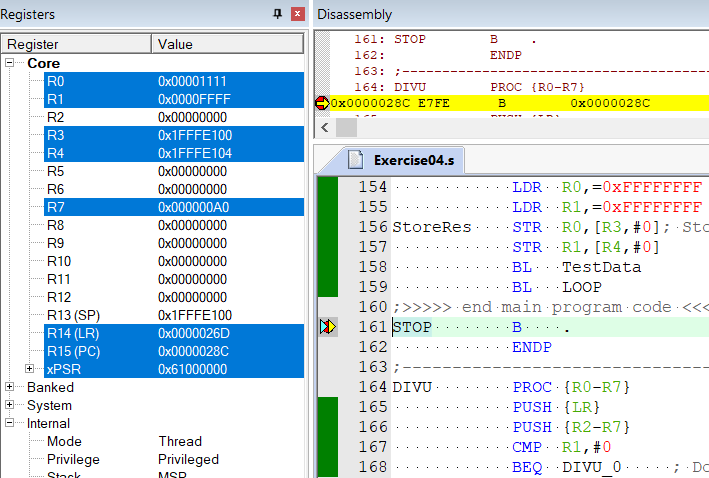
\includegraphics[width=\textwidth]{cap1}
	\caption{Debugger results after program execution.}
	\label{fig:capture1}
\end{figure}

Figure \ref{fig:capture1} shows the register values after program execution.
The important register to note is R6 which is used by \code{TestData} as
the an error output. This capture shows that a valid \code{DIVU} was written
as the value of R6 indicates to errors occured.
\pagebreak

Another screen capture was taken of the memory map after compiling the
assembly code to determine the memory regions of the generated machine-code.

\begin{figure}[h!]
	\centering
	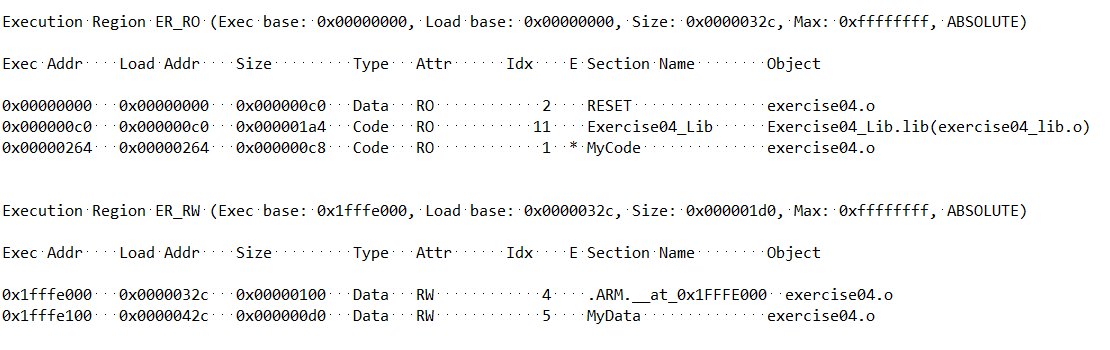
\includegraphics[width=\textwidth]{cap2}
	\caption{Memory map of the assembly program.}
	\label{fig:capture2}
\end{figure}

The code written for the main program is labelled \code{MyCode} starting
at \code{0x264}. According to the map file this section has a size of \code{0xc8} or $200$ bytes. This however includes the instruction inside
the \code{DIVU} subroutine. Looking at the listing file shows that the 
final instruction in the main part of the program:

\begin{lstlisting}
162 0000002A                 ENDP
\end{lstlisting}

This line tells us that the offset of the final instruction in the main
of the program is \code{0x2A} meaning that the main program has a size of
$42$ bytes. The ending address address of \code{MyCode} is
\code{0x000002A6}.

The \code{Exercise04\_Lib} which includes the \code{InitData}, 
\code{LoadData} and \code{TestData} subroutines starts at \code{0xC0}
and ends \code{0x264} with a size of $420$ bytes. 

Looking at the assembly source code, the section directly before the 
\code{MyData} section labelled \code{.ARM.\_\_at\_0x1FFFE000} holds the
stack data. The symbol \code{\_\_initial\_sp} is defined at the end of this
section because the stack grows upward toward the beginning of the memory
area. The stack's size is defined by an \code{EQU} to be 0x100 or 256 bytes.
The stack area starts at \code{0x1FFFE000} and ends at \code{0x1FFFE100}.

The section after the stack area (\code{MyData} starts where the stack 
ends at \code{0x1FFFE100}. This section holds the variables $P$, $Q$, 
and the $Results$ array. $P$ and $Q$ are both word variables. The 
$Results$ array contains $2 \cdot MaxData$ word variables where $MaxData$
is defined at $25$. Therefore the size of \code{MyData} is $208$ bytes
or \code{0xD0}. This section ends at the \code{0x1FFFE1D0} address.


\section*{Conclusion}
This lab exercise successfully introduced students to the use of 
subroutines and linking external libraries. In addition to this it taught
students how to implement binary unsigned integer division. This lab
exercise was successful as the subroutine to verify the results of the 
division subroute did not indicate any errors were found.


\label{LastPage}
\end{document}
